\section{Gated RNNs: LSTM and GRU}
\begin{frame}{}
    \LARGE Recurrent Neural Networks: \textbf{Gated Units: LSTM \& GRU}
\end{frame}

\begin{frame}{The Problem: Long-Term Dependencies}
    \begin{columns}
        \begin{column}{0.46\textwidth}
            The vanilla (Elman) RNN written out:
            \begin{align*}
                h_t & = \tanh(W_{hh} h_{t-1} + W_{xh} x_t + b_h) \\
                y_t & = W_{hy} h_t + b_y
            \end{align*}
            \begin{itemize}
                \item The same $W_{hh}$, $W_{xh}$, $W_{hy}$ are reused at every time step.
                \item Backpropagating from $h_T$ back to $h_1$ multiplies by $W_{hh}^{\top}$ once per step.
            \end{itemize}
        \end{column}
        \begin{column}{0.54\textwidth}
            \begin{itemize}
                \item That product of $T-1$ copies of one matrix decides whether the gradient survives:
                      \begin{itemize}
                          \item largest singular value of $W_{hh} > 1$: \textbf{exploding} gradients;
                          \item largest singular value $< 1$: \textbf{vanishing} gradients.
                      \end{itemize}
                \item Exploding gradients have a cheap fix, \textbf{gradient clipping}: rescale the
                      gradient whenever its norm exceeds a threshold.
                \item Vanishing gradients do not, so plain RNNs struggle to connect information across
                      many time steps.
                \item \textbf{Idea:} add gating mechanisms that let the network \emph{choose} what to keep, forget, and output.
            \end{itemize}
        \end{column}
    \end{columns}
\end{frame}

\begin{frame}{Long Short-Term Memory (LSTM)}
    \begin{columns}
        \begin{column}{0.55\textwidth}
            \begin{itemize}
                \item Maintains a separate \textbf{cell state} $c_t$ that acts as a memory ``conveyor
                      belt''.
                \item Three gates control the flow of information:
                      \begin{itemize}
                          \item \textbf{Forget gate} $f_t$: what to erase from memory.
                          \item \textbf{Input gate} $i_t$: what new information to store.
                          \item \textbf{Output gate} $o_t$: what to expose as the hidden state.
                      \end{itemize}
                \item Additive cell updates create a gradient ``highway'', easing long-range
                      learning.
            \end{itemize}
        \end{column}
        \begin{column}{0.45\textwidth}
            \small
            \begin{align*}
                f_t         & = \sigma(W_f [h_{t-1}, x_t] + b_f)          \\
                i_t         & = \sigma(W_i [h_{t-1}, x_t] + b_i)          \\
                o_t         & = \sigma(W_o [h_{t-1}, x_t] + b_o)          \\
                \tilde{c}_t & = \tanh(W_c [h_{t-1}, x_t] + b_c)           \\
                c_t         & = f_t \odot c_{t-1} + i_t \odot \tilde{c}_t \\
                h_t         & = o_t \odot \tanh(c_t)
            \end{align*}
        \end{column}
    \end{columns}
\end{frame}

\begin{frame}{Gated Recurrent Unit (GRU)}
    \begin{columns}
        \begin{column}{0.55\textwidth}
            \begin{itemize}
                \item A lighter alternative to the LSTM with \textbf{two} gates and no separate cell
                      state.
                \item \textbf{Reset gate} $r_t$: how much past state to ignore.
                \item \textbf{Update gate} $z_t$: how much to blend old and new state.
                \item Fewer parameters $\Rightarrow$ faster to train, often with comparable accuracy.
            \end{itemize}
        \end{column}
        \begin{column}{0.45\textwidth}
            \small
            \begin{align*}
                z_t         & = \sigma(W_z [h_{t-1}, x_t])                     \\
                r_t         & = \sigma(W_r [h_{t-1}, x_t])                     \\
                \tilde{h}_t & = \tanh(W [r_t \odot h_{t-1}, x_t])              \\
                h_t         & = (1 - z_t)\odot h_{t-1} + z_t \odot \tilde{h}_t
            \end{align*}
        \end{column}
    \end{columns}
\end{frame}

\begin{frame}{LSTM vs GRU}
    \begin{figure}
        \centering
        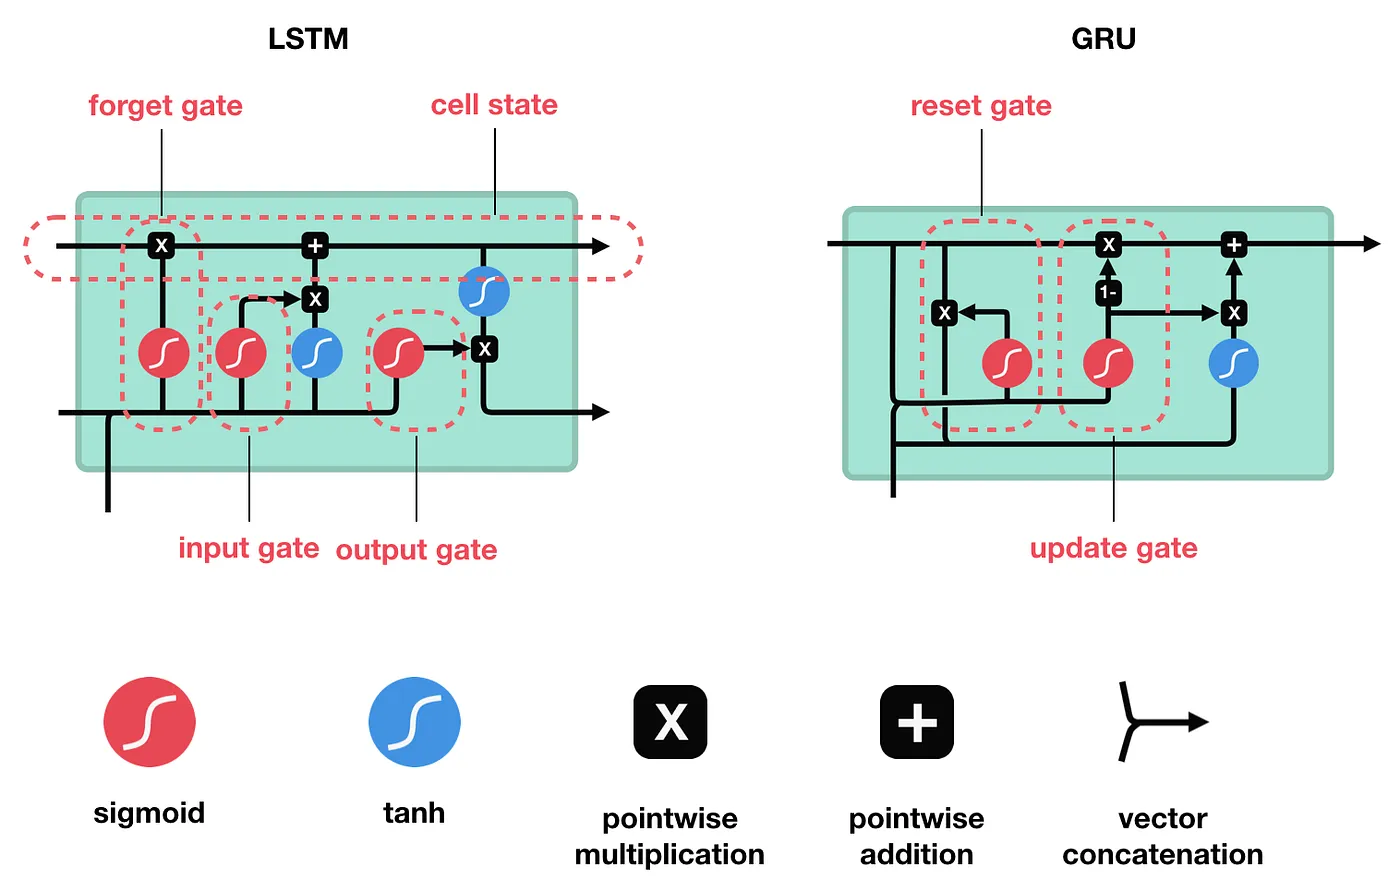
\includegraphics[width=0.8\textwidth,height=0.8\textheight,keepaspectratio]{images/rnn-lstm-gru/lstm_gru_cells.png}
        \caption*{\tiny Source: Michael Phi, \href{https://medium.com/data-science/illustrated-guide-to-lstms-and-gru-s-a-step-by-step-explanation-44e9eb85bf21}{Illustrated Guide to LSTM's and GRU's: A step by step explanation}}
    \end{figure}
\end{frame}

\begin{frame}{LSTM vs GRU}
    \begin{table}[]
        \centering
        \begin{tabular}{|l|c|c|}
            \hline
            \textbf{Aspect}     & \textbf{LSTM}             & \textbf{GRU}                 \\
            \hline
            Gates               & 3 (input, forget, output) & 2 (reset, update)            \\
            Separate cell state & Yes                       & No                           \\
            Parameters          & More                      & Fewer                        \\
            Training speed      & Slower                    & Faster                       \\
            Typical use         & Long, complex sequences   & Smaller data / faster models \\
            \hline
        \end{tabular}
    \end{table}
    \vspace{0.5cm}
    \begin{itemize}
        \item Both dramatically outperform vanilla RNNs on long-range dependencies.
        \item The choice is empirical: GRU is a strong, cheaper default, while LSTM can edge
              ahead on hard tasks.
    \end{itemize}
\end{frame}
